%%%%%%%%%%%%%%%%%%%%%%%%%%%%%%%%%%%%%%%%%
% Simple Sectioned Essay Template
% LaTeX Template
%
% This template has been downloaded from:
% http://www.latextemplates.com
%
% Note:
% The \lipsum[#] commands throughout this template generate dummy text
% to fill the template out. These commands should all be removed when 
% writing essay content.
%
%%%%%%%%%%%%%%%%%%%%%%%%%%%%%%%%%%%%%%%%%

%----------------------------------------------------------------------------------------
%	PACKAGES AND OTHER DOCUMENT CONFIGURATIONS
%----------------------------------------------------------------------------------------
\documentclass[12pt]{article} % Default font size is 12pt, it can be changed here

\usepackage{geometry} % Required to change the page size to A4
\geometry{a4paper} % Set the page size to be A4 as opposed to the default US Letter

\usepackage{graphicx} % Required for including pictures
\usepackage{subcaption}
\captionsetup{compatibility=false}
\usepackage{float} % Allows putting an [H] in \begin{figure} to specify the exact location of the figure
\usepackage{wrapfig} % Allows in-line images such as the example fish picture

\usepackage{mathtools}

\usepackage{hyperref}


\usepackage{fancyhdr}
\pagestyle{fancy}
\fancyhf{}
%\fancyhead[LE,RO]{Share\LaTeX}
\fancyhead[RE,LO]{Pixel-based Skin Color Detection Techniques}
\fancyfoot[CE,CO]{Master's in Computer Vision and Robotics, University of Burgundy}
\fancyfoot[LE,RO]{\thepage}
\renewcommand{\headrulewidth}{1.5pt}
\renewcommand{\footrulewidth}{1pt}
 

%\usepackage{lipsum} % Used for inserting dummy 'Lorem ipsum' text into the template

\linespread{1.1} % Line spacing

%\setlength\parindent{0pt} % Uncomment to remove all indentation from paragraphs

\graphicspath{{Pictures/}} % Specifies the directory where pictures are stored

% Defining tikz for flow chart
\usepackage{tikz}
\usetikzlibrary{shapes.geometric, arrows}

\tikzstyle{PointCloud} = [rectangle, rounded corners, minimum width=3cm, minimum height=1cm,text centered, text width=3cm, draw=black, fill=red!30]
\tikzstyle{Processes} = [rectangle, minimum width= 4.5cm, minimum height=1.1 cm,text centered, draw=black, fill=orange!30]
\tikzstyle{arrow} = [thick,->,>=stealth]


\usepackage{caption}
\usepackage{subcaption}
\usepackage{listings}
\usepackage{color} %red, green, blue, yellow, cyan, magenta, black, white
\definecolor{mygreen}{RGB}{28,172,0} % color values Red, Green, Blue
\definecolor{mylilas}{RGB}{170,55,241}

\lstset{language=Matlab,%
	basicstyle=\footnotesize\ttfamily,
	breaklines=true,%
	morekeywords={matlab2tikz},
	keywordstyle=\color{blue},%
	morekeywords=[2]{1}, keywordstyle=[2]{\color{black}},
	identifierstyle=\color{black},%
	stringstyle=\color{mylilas},
	commentstyle=\color{mygreen},%
	showstringspaces=false,%without this there will be a symbol in the places where there is a space
	numbers=left,%
	numberstyle={\tiny \color{black}},% size of the numbers
	numbersep=9pt, % this defines how far the numbers are from the text
	emph=[1]{for,end,break},emphstyle=[1]\color{red}, %some words to emphasise
	%emph=[2]{word1,word2}, emphstyle=[2]{style},    
}


\begin{document}

%----------------------------------------------------------------------------------------
%	TITLE PAGE
%----------------------------------------------------------------------------------------

\begin{titlepage}

\newcommand{\HRule}{\rule{\linewidth}{0.5mm}} % Defines a new command for the horizontal lines, change thickness here

\center % Center everything on the page

\textsc{\LARGE Image Processing Final Project}\\[1cm] % Name of your university/college
\textsc{\Large University of Burgundy}\\[0.8cm] % Major heading such as course name
\textsc{\large Master's in Computer Vision and Robotics}\\[0.5cm] % Minor heading such as course title
\textsc{\large (VIBOT \& MScV)}\\[0.8cm] % Minor heading such as course title

\HRule \\[0.8cm]
{ \huge \bfseries Pixel-based Skin Color Detection Techniques}\\[0.4cm] % Title of your document
\HRule \\[2cm]

\begin{minipage}{0.5\textwidth}
\begin{flushleft} \large
\emph{Group members:}\\
% Add names if you want
 %Yu \textsc{Liu}  \\ 
 Hassa ZAAL \\
 AbdelRahman ABUBAKR\\

\end{flushleft}
\end{minipage}
~
\begin{minipage}{0.4\textwidth}
\begin{flushright} \large
\emph{Supervisor:} \\
Prof. Desire Sedibe  % Supervisor's Name
\end{flushright}
\end{minipage}\\[3 cm]

%{\large \today}\\[1cm] % Date, change the \today to a set date if you want to be precise


\includegraphics{Logo}\\[0cm] % Include a department/university logo - this will require the graphicx package

% \vfill % Fill the rest of the page with whitespace

\end{titlepage}

%----------------------------------------------------------------------------------------
%	TABLE OF CONTENTS 
%----------------------------------------------------------------------------------------

 \tableofcontents % Include a table of contents

\newpage % Begins the essay on a new page instead of on the same page as the table of contents 

%----------------------------------------------------------------------------------------
%	INTRODUCTION
%----------------------------------------------------------------------------------------
\section{Introduction} % Major section

Human skin color has been used and proved to be an effective feature in many applications such as human face detection, hand tracking, image content filtering, content-aware video compression and many more. In this project we implemented the algorithms mentioned in the paper "A Survey on Pixel-Based Skin Color Detection Techniques" by Vladimir Vezhnevets, Vassili Sazonov, and Alla Andreeva.

\subsection{UCI skin segmentation data set}

The Authors of the paper mentioned using the Compaq skin database for comparing the results of all algorithms. However, we could not find any source for the Compaq database, therefore we decided to use the UCI skin segmentation dataset, provided by Center for Machine Learning and Intelligent Systems at University of California, Irvine. the dataset can be downloaded from here:
\href{https://archive.ics.uci.edu/ml/datasets/Skin+Segmentation}{https://archive.ics.uci.edu/ml/datasets/Skin+Segmentation} \\

According to the dataset website, the skin dataset is collected by randomly sampling B,G,R values from face images of various age groups (young, middle, and old), race groups (white, black, and asian), and genders obtained from FERET database and PAL database. Total learning sample size is 245057; out of which 50859 is the skin samples and 194198 is non-skin samples.\\

This dataset is of the dimension 245057 * 4 where first three columns are B,G,R values and fourth column is of the class labels (decision variable y), in the dataset file Skin colors are labeled as number 1 and Nonskin elements as 2.

\subsection{Dataset visualization}
First step to start any project with big amount of data, is to visualize this data to see its distribution and roughly expect the behavior of your algorithms. for our data set, we wrote a simple code Plot-Dataset.py that plots skin data in blue, and nonskin in red, the 2 axes are the Cb and Cr components of the colors. Figure shows the visualization of the dataset. 

\begin{figure}[H]
		\centering
		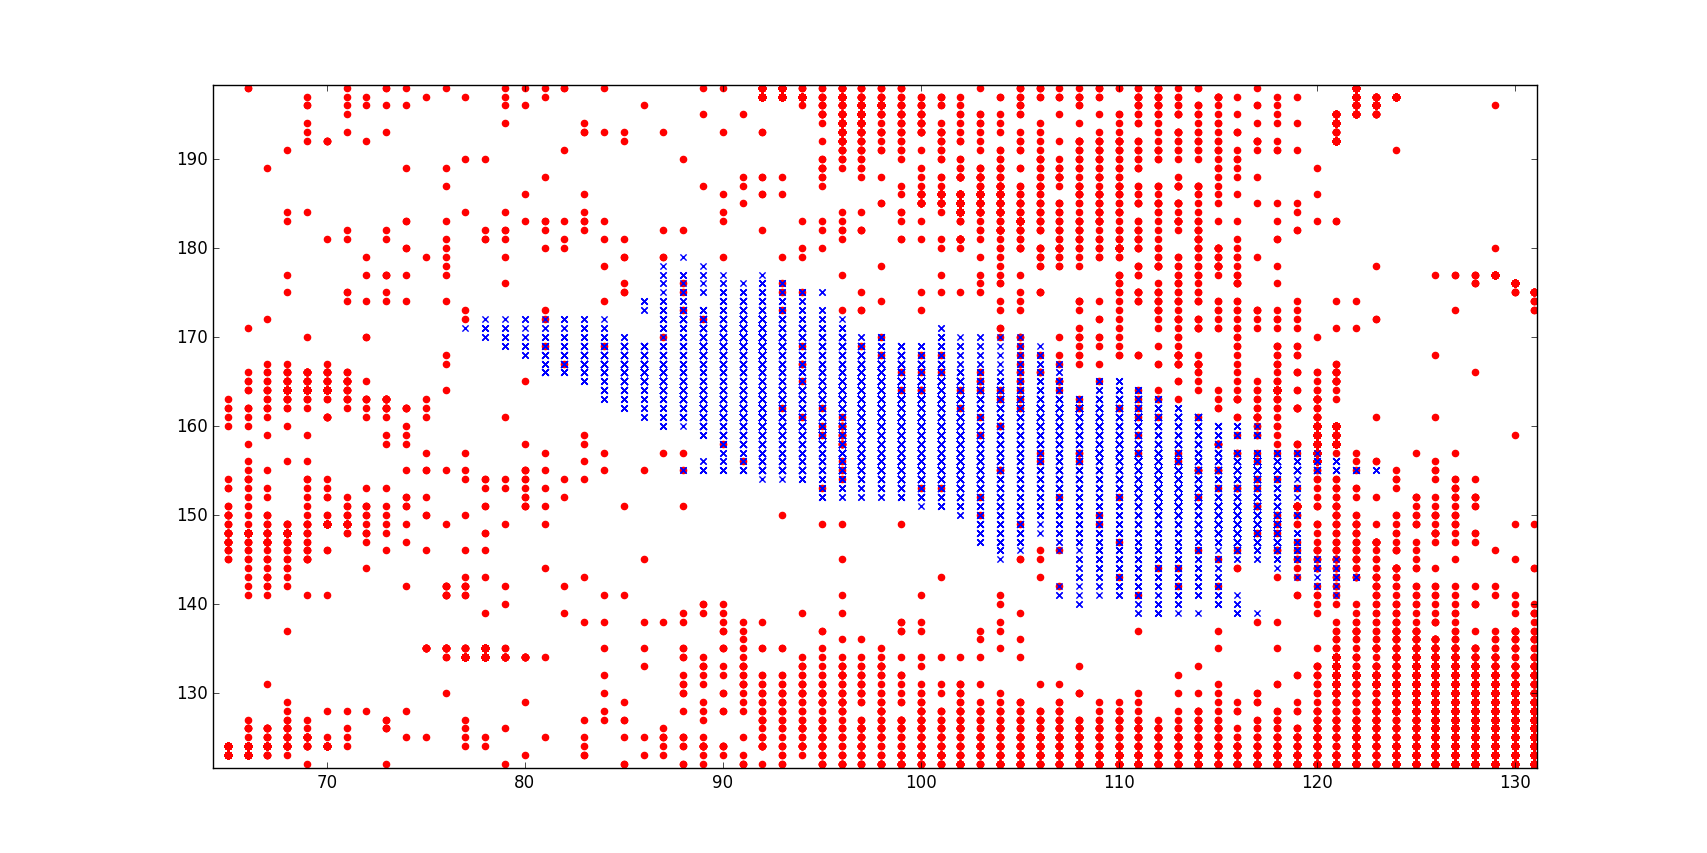
\includegraphics[width=\textwidth]{Skin-Nonskin-zoomed.png}
		\caption{UCI Data set visualization}	
\end{figure}

\subsection{How to run ?}
For the code implementation we used Python 3.5, with some help from Scikit-Learn 0.18.1 library when needed. We put all the algorithms in different files, and different directories, so for running any code, you can use any python IDE, or by Linux terminal change the directory for the code directory, then write:

\hspace*{\fill}
        Python  FileName.py
\hspace*{\fill} \\


%\\
All source code is available on Github Repository:
\href{https://github.com/abdelrahman-gaber/Pixel-based-Skin-Color-Detection}{https://github.com/abdelrahman-gaber/Pixel-based-Skin-Color-Detection } 


\section{Explicitly defined skin region} 
One method to build a skin classifier is to define explicitly (through a number of rules) the boundaries skin cluster in some color space. Any (R, G, B) pixel values given to the algorithm is classified as skin if:

$$ R > 95 \: and   \: G > 40  \: and  \: B > 20  \: and $$ 
$$max(R, G, B) - min(R, G, B) > 15  \: and $$
$$|R − G| > 15  \: and  \: R > G  \: and  \: R > B $$

This algorithm is implemented in the file defined-skin-region.py, and the results was as follows:

\begin{center}
True positive rate = 100\% \\
False Positive rate = 3.7\%
\end{center}   

We notice here the big value of True positive rate, but this is expected as the data set used has an obvious boundary for the skin region. 


\section{Non-parametric skin distribution modeling} % Major section
The final goal of skin color detection is to build a decision rule, that will discriminate between skin and non-skin pixels. This is usually accomplished by introducing a metric, which measures distance (in general sense) of the pixel color to skin tone. The type of this metric is defined by the skin color modeling method. the paper differentiated between many types of modeling, the most important two of them are Non-parametric and parametric skin modeling techniques.\\

The key idea of the non-parametric skin modelling methods is to es-
timate skin color distribution from the training data without deriving an explicit model of the skin color. The result of these methods sometimes is referred to as construction of Skin Probability Map (SPM).

\subsection{Bayes Classifier} 
Naive Bayes methods are a set of supervised learning algorithms based on applying Bayes’ theorem with the “naive” assumption of independence between every pair of features. Given the vectors of the RGB colors with the class labels of them, we used the Scikit-Learn Naive Bayes classifier to train and test our data. \\

We used half of the elements of both skin and nonskin data for the training, and the other half for the test.The Naive Bayes classifier has many different types, the different classifiers differ mainly by the assumptions they make regarding the distribution of $P(x_i| y)$. For our case, as we know that the data is mainly a gaussian type, so we used the GaussianNB() function, which implements the Gaussian Naive Bayes algorithm for classification. In this case, the likelihood of the features is assumed to be Gaussian. \\

The result of Naive bayes classifier for our labeled data is as follows:


\begin{center}
True positive rate = 99.032\% \\
False Positive rate = 0.967\%
\end{center}



\section{Parametric skin distribution modeling} % Major section

The need for more compact skin model representation for certain applications along with ability to generalize and interpolate the training data stimulates the development of parametric skin distribution models.

All implemented parametric methods operate in colorspace chrominance plane, ignoring the luminance information. For our code we convert the RGB color data to YCbCr first, then work on Cb and Cr values. 


\subsection{Single Gaussian model } 

Skin color distribution can be modeled by an elliptical Gaussian
joint probability density function (pdf), for this case we implemented the joint pdf between Cb and Cr components, and used half of the skin elements to train the model and find the parameters. Figure 2 shows a visualization of our Gaussian model, where the X axis is the Cb component, and Y axis is the Cr component. \\

The mean values and the covariance matrix of our model are as follows:

$$
Mean =  \begin{bmatrix}
  100.48 & 161.55
 \end{bmatrix}
$$
$$
Covariance =  \begin{bmatrix}
  73.87 & -43.02 \\
  -43.02 & 39.52 
 \end{bmatrix}
$$

After training the model and getting the parameters, we set a threshold to the probability of any new color input. for each input from the test set, if the probability is bigger than the threshold, the color input is considered as skin, otherwise, it is non-skin pixel. for our case we chosed a probability threshold = 0.0001, and the results of the testing set are as follows:

\begin{center}
True positive rate = 98.50\% \\
False Positive rate = 0.16\%
\end{center}   

We notice the high value of True poisitve, and low value of False Positive rates. This can be explained from the visualization of the original data set, from which it is obvious that the skin and non-skin data are not overlapped, and there is an obvious boundry between them.

\begin{figure}[H]
		\centering
		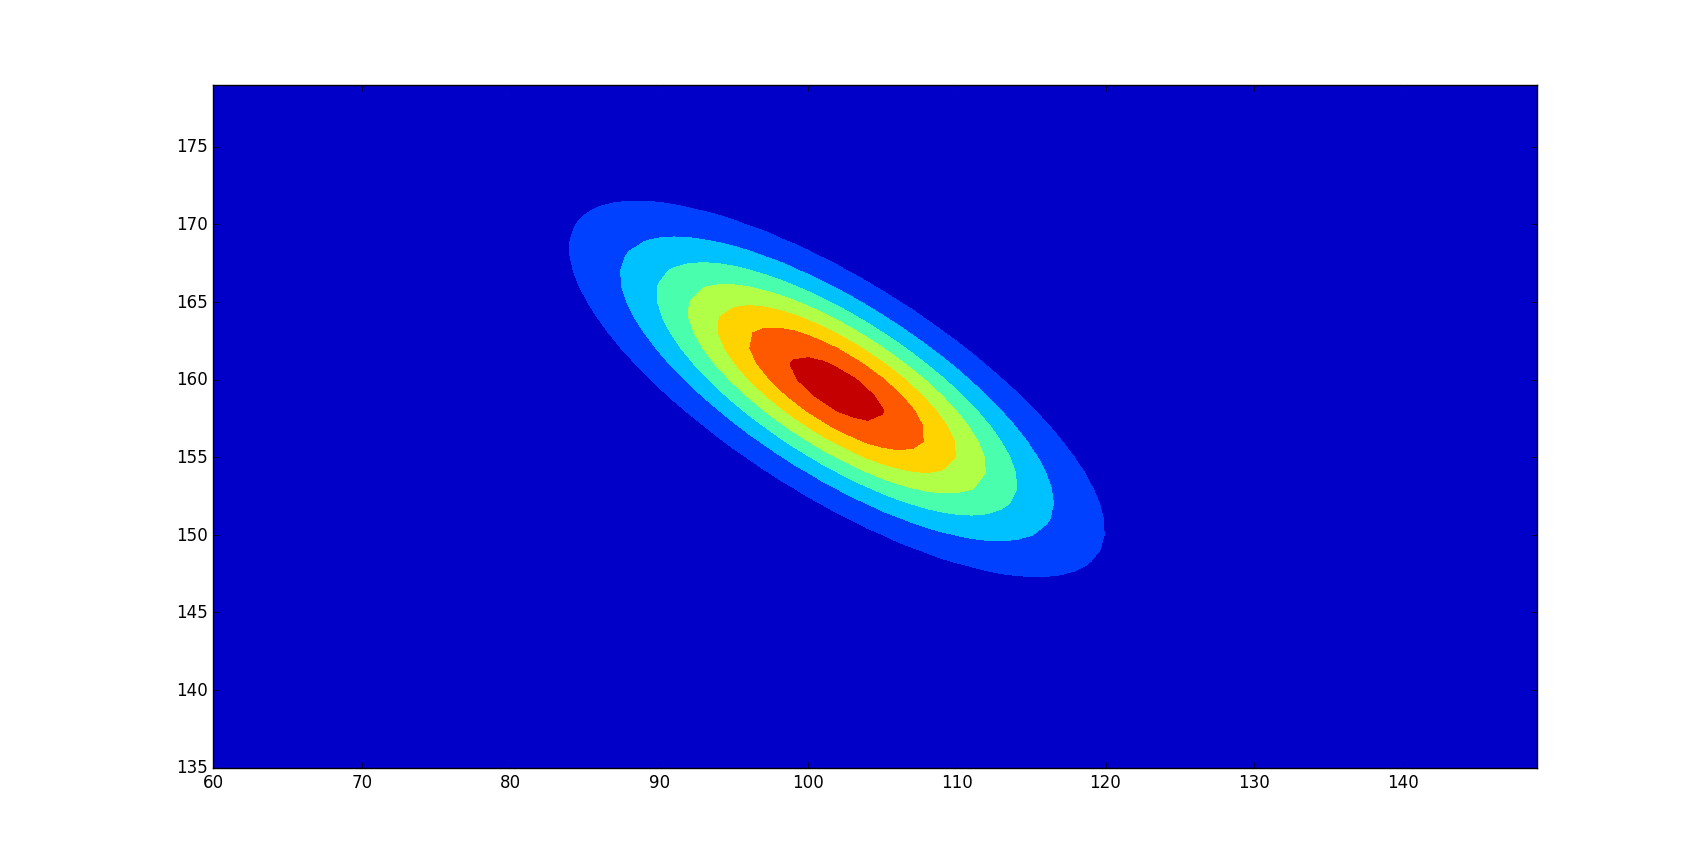
\includegraphics[width=\textwidth]{Gaussian-model.png}
		\caption{The Gaussian Model of the skin data}	
\end{figure}


\subsection{Gaussian Mixture Model (GMM)}

A more sophisticated model, capable of describing complex-shaped
distributions is the Gaussian mixture model. It is the generalization of the single Gaussian, the pdf in this case is just a sum of many weighted Gaussian each with its own mean and covariance. The difficulty of  this model arises when trying to find the parameters of each Gaussian, and the weight of each of them. In our case we used the Expectation Maximization algorithm to find all these parameters. \\

To implement this algorithm and find the parameters from the training data, we used the Scikit-Learn mixture package, which implements Gaussian Mixture Model, and finds the parameters using EM algorithm. For our training data, we tried various number of Gaussians and discovered that the best number of them is 4, which increases the TP vs. FP values, and balance the weights of the Gaussians. Figure 3 shows the visualization of the GMM model with 4 components, we can observe that some Gaussians have more probability weight than others [Red color], these weights are also evaluated by the EM algorithm. 

\begin{figure}[H]
		\centering
		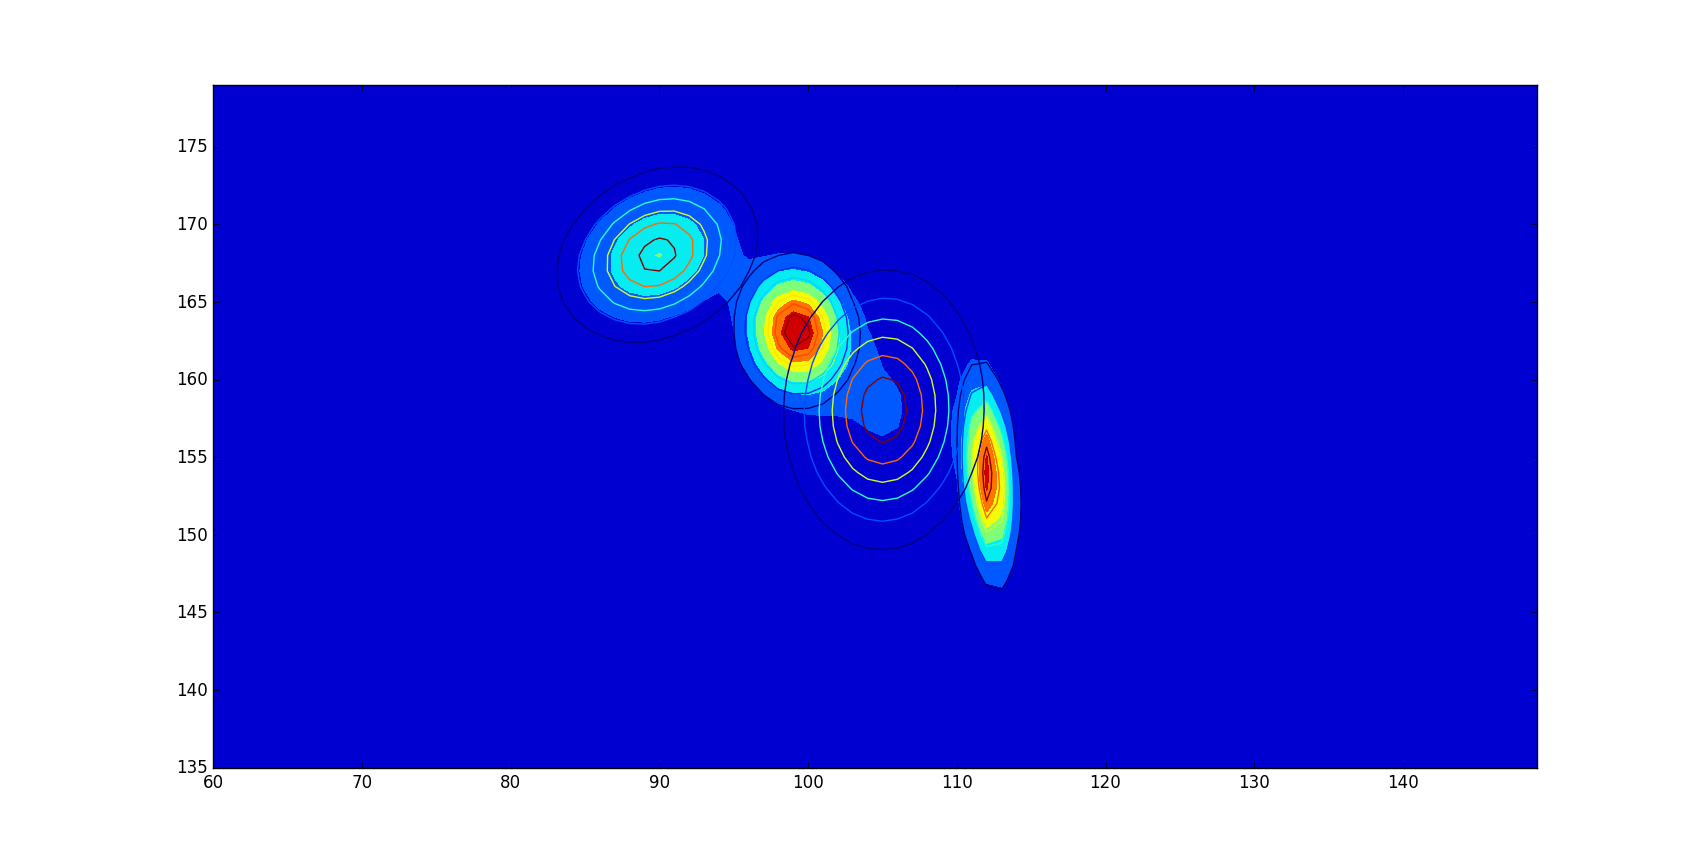
\includegraphics[width=\textwidth]{GMM_4.png}
		\caption{The Gaussian Mixture Model obtained by EM algorithm}	
\end{figure}

Using the EM algorithm, we found the parameters of the Gaussians as follows:\\
First component with weight = 0.230 and 
$$
Mean_1 =  \begin{bmatrix}
  112.10 & 153.82
 \end{bmatrix}
$$
$$
Covariance_1 =  \begin{bmatrix}
  1.13 & -1.05 \\
  -1.05& 14.45
 \end{bmatrix}
$$


Second component with weight = 0.328 and 
$$
Mean_2 =  \begin{bmatrix}
  99.21 & 163.13
 \end{bmatrix}
$$
$$
Covariance_2 =  \begin{bmatrix}
  4.32 & -0.27 \\
  -0.27 &  6.10
 \end{bmatrix}
$$


Third component with weight = 0.159 and 
$$
Mean_2 =  \begin{bmatrix}
  105.09970179 & 158.0579959
 \end{bmatrix}
$$
$$
Covariance_2 =  \begin{bmatrix}
  11.84&  0.38 \\
  0.38 &  21.36
 \end{bmatrix}
$$


Fourth component with weight = 0.281 and 
$$
Mean_2 =  \begin{bmatrix}
  89.84 & 168.04
 \end{bmatrix}
$$
$$
Covariance_2 =  \begin{bmatrix}
  12.11 & 2.18 \\
  2.18 & 8.42
 \end{bmatrix}
$$

An important thing to notice is that the sum of all weights must be = 1, as the model is a new pdf. For any new color vector, we can now compare its probability with a threshold, and it is considered as color if the probability is bigger than this threshold. For our code, we set the threshold to value = 0.000001. For this case the results of the testing set are as follows:


\begin{center}
True positive rate = 92.48\% \\
False Positive rate = 0.169\%
\end{center}


\subsection{Elliptic boundary model}
By examining skin and non-skin distributions in several colorspaces, it has been concluded that skin color cluster, being approximately elliptic in shape is not well enough approximated by the single Gaussian model. Due to asymmetry of the skin cluster with respect to its density peak, usage of the symmetric Gaussian model leads to high false positives rate. An alternative called an ”elliptical boundary model” is equally fast and simple in training and evaluation as the single Gaussian model, and avoid the complexity and time consumption taken by Gaussian Mixture Model. \\

The algorithm is implemented by the equations in section 3.34 in the paper, and all the parameters of the model are evaluated. Given threshold $\theta$ and input chrominance of a pixel X, the pixel is classified as skin if  $\Phi$(X) $<$  $\theta$ and as non-skin otherwise. For our code, we found a threshold of value = 1.0 is good choice. the results of the testing set are as follows:

\begin{center}
True positive rate = 98.682\% \\
False Positive rate = 0.205\%
\end{center}




%----------------------------------------------------------------------------------------
%	BIBLIOGRAPHY >> If there are references
%----------------------------------------------------------------------------------------
%\begin{thebibliography}{99} % Bibliography - this is intentionally simple in this template

%\bibitem[Figueredo and Wolf, 2009]{Figueredo:2009dg} Figueredo, A.~J. and Wolf, P. S.~A. (2009).

%\newblock Assortative pairing and life history strategy - a cross-cultural  study.
%\newblock {\em Human Nature}, 20:317--330.
 
%\end{thebibliography}

%----------------------------------------------------------------------------------------

\end{document}